% This contents of this file will be inserted into the _Solutions version of the
% output tex document.  Here's an example:

% If assignment with subquestion (1.a) requires a written response, you will
% find the following flag within this document: <SCPD_SUBMISSION_TAG>_1a
% In this example, you would insert the LaTeX for your solution to (1.a) between
% the <SCPD_SUBMISSION_TAG>_1a flags.  If you also constrain your answer between the
% START_CODE_HERE and END_CODE_HERE flags, your LaTeX will be styled as a
% solution within the final document.

% Please do not use the '<SCPD_SUBMISSION_TAG>' character anywhere within your code.  As expected,
% that will confuse the regular expressions we use to identify your solution.

\def\assignmentnum{1 }
\def\assignmentname{Foundations}
\def\assignmenttitle{XCS221 Assignment \assignmentnum --- \assignmentname}
\input{macros}
\begin{document}
\pagestyle{myheadings} \markboth{}{\assignmenttitle}

% <SCPD_SUBMISSION_TAG>_entire_submission

This handout includes space for every question that requires a written response.
Please feel free to use it to handwrite your solutions (legibly, please).  If
you choose to typeset your solutions, the |README.md| for this assignment includes
instructions to regenerate this handout with your typeset \LaTeX{} solutions.
\ruleskip

\LARGE
1.a
\normalsize

% <SCPD_SUBMISSION_TAG>_1a
\begin{answer}
  % ### START CODE HERE ###
  % NumPy tutor session transcript (interactive, 15-20 min).
  % CHECK: open the link in a private window before submitting to confirm the
  % share is public and the transcript loads.
  Link to my NumPy tutoring session:
  \url{https://claude.ai/share/9365fd54-617b-4519-875c-ed96bf982080}
  % ### END CODE HERE ###
\end{answer}
% <SCPD_SUBMISSION_TAG>_1a

\LARGE
1.b
\normalsize
% <SCPD_SUBMISSION_TAG>_1b
\begin{answer}
  % ### START CODE HERE ###
  \textbf{Answer:} $O(mnp)$.

  \medskip
  \textbf{Justification.} The product $C = AB$ has $m \cdot p$ entries, and each operation is an
  inner product of length $n$:
  so each operation costs $n$ multiply--adds. The total is therefore $mp \cdot n = O(mnp)$.

  % ### END CODE HERE ###
\end{answer}
% <SCPD_SUBMISSION_TAG>_1b

\LARGE
1.c
\normalsize
% <SCPD_SUBMISSION_TAG>_1c
\begin{answer}
  % ### START CODE HERE ###
  % einsum / einops tutor session transcript (interactive, 15-20 min).
  % CHECK: open the link in a private window before submitting to confirm the
  % share is public and the transcript loads.
  Link to my einops tutoring session:
  \url{https://claude.ai/share/f6b32ebe-894a-4ff8-b7a5-2ff4666d93cf}
  % ### END CODE HERE ###
\end{answer}
% <SCPD_SUBMISSION_TAG>_1c

\LARGE
1.d
\normalsize
% <SCPD_SUBMISSION_TAG>_1d
\begin{answer}
  % ### START CODE HERE ###
  \textbf{(i) $Xw$, shapes $(n,d), (d,) \to (n,)$}
  \[
    \texttt{einsum(X, w, 'n d, d -> n')}
  \]
  The single axis of $w$ is labelled \texttt{d} so that it aligns with the column axis of $X$.
  Since \texttt{d} is absent from the output it is summed over, giving
  $(Xw)_i = \sum_d X_{id} w_d$. The axis \texttt{n} is carried through, so the result has one
  entry per row of $X$.

  \medskip
  \textbf{(ii) $XX^\top$, shapes $(n,d), (n,d) \to (n,n)$}
  \[
    \texttt{einsum(X, X, 'i d, j d -> i j')}
  \]
  Entry $[i,j]$ is the dot product of row $i$ with row $j$, that is
  $(XX^\top)_{ij} = \sum_d X_{id} X_{jd}$. The two row axes index \emph{different} rows, so they were assigned differentletters \texttt{i} and \texttt{j}, both of which are kept in the output.
  The feature axis \texttt{d} is shared by both operands and dropped from the output, so it is
  summed over.

  \medskip
  \textbf{(iii) $\operatorname{diag}(X^\top X)$, shapes $(n,d), (n,d) \to (d,)$}
  \[
    \texttt{einsum(X, X, 'n d, n d -> d')}
  \]
  Using the same index letter for the column axis of both inputs forces the row and column index of $X^\top X$ to be equal, which selects the diagonal entries: $y[d] \mathrel{+}= X[n,d] \cdot X[n,d]$,
  each entry squared and added into its own column's position on the output vector. The $n$ axis is contracted away because it is not named in the output.
 

  % ### END CODE HERE ###
\end{answer}
% <SCPD_SUBMISSION_TAG>_1d

\clearpage

\LARGE
2.a
\normalsize

% <SCPD_SUBMISSION_TAG>_2a
\begin{answer}
  % ### START CODE HERE ###
  \textbf{Gradient.} $\nabla f(\mathbf w) = 2(\mathbf w - \mathbf c)$.

  \medskip
  \textbf{Derivation.} Differentiation is linear, so it moves inside the sum:
  \[
    \frac{\partial f}{\partial w_j}
      \;=\; \frac{\partial}{\partial w_j}\sum_{i=1}^{d}(w_i-c_i)^2
      \;=\; \sum_{i=1}^{d}\frac{\partial}{\partial w_j}(w_i-c_i)^2 .
  \]
  The function is \emph{separable}: the term indexed by $i$ involves only $w_i$. Every term with
  $i \neq j$ is therefore a constant with respect to $w_j$ and differentiates to zero, so only the
  $i = j$ term survives. Applying the chain rule to that one term, and using
  $\frac{d}{dw_j}(w_j-c_j) = 1$ since $c_j$ is constant,
  \[
    \frac{\partial f}{\partial w_j} \;=\; 2(w_j-c_j).
  \]
  Every component has the same form, so stacking them gives
  \[
    \nabla f(\mathbf w) \;=\; 2(\mathbf w - \mathbf c).
  \]

  \medskip
  \textbf{Evaluated at $\mathbf w = \mathbf 0$.}
  \[
    \nabla f(\mathbf 0) \;=\; 2(\mathbf 0 - \mathbf c) \;=\; -2\mathbf c .
  \]
  % ### END CODE HERE ###
\end{answer}
% <SCPD_SUBMISSION_TAG>_2a

\LARGE
2.c
\normalsize

% <SCPD_SUBMISSION_TAG>_2c
\begin{answer}
  % ### START CODE HERE ###
  % Working notes kept for reference (not rendered):
  %   ds/dA entries are the ROW sums of B; ds/dB entries are the COLUMN sums of A.
  %   Each gradient has the same shape as the matrix it differentiates against.
  \textbf{Product.} Each entry of $C$ is one row of $A$ against one column of $B$:
  \[
    \begin{aligned}
      C_{11} &= 2\cdot 7 + 1\cdot 9 + 3\cdot 1 = 26, &\qquad
      C_{12} &= 2\cdot 8 + 1\cdot 0 + 3\cdot 2 = 22, \\
      C_{21} &= 4\cdot 7 + 5\cdot 9 + 6\cdot 1 = 79, &\qquad
      C_{22} &= 4\cdot 8 + 5\cdot 0 + 6\cdot 2 = 44,
    \end{aligned}
  \]
  so
  \[
    C = AB = \begin{pmatrix} 26 & 22 \\ 79 & 44 \end{pmatrix},
    \qquad
    s = 26 + 22 + 79 + 44 = 171 .
  \]

  \medskip
  \textbf{Gradient with respect to $A$.} Since $s$ sums every entry of $C$ exactly once,
  $\frac{\partial s}{\partial C_{i,j}} = 1$ for all $i,j$, and $C_{i,j} = \sum_k A_{i,k} B_{k,j}$, so
  \[
    \frac{\partial s}{\partial A_{i,k}}
      = \sum_j \frac{\partial s}{\partial C_{i,j}} \cdot B_{k,j}
      = \sum_j B_{k,j},
  \]
  the row sums of $B$: $7+8=15$, $9+0=9$, $1+2=3$. Every row of $A$ meets the same rows of $B$, so
  the result repeats down both rows:
  \[
    \frac{\partial s}{\partial A} = \begin{pmatrix} 15 & 9 & 3 \\ 15 & 9 & 3 \end{pmatrix}.
  \]

  \medskip
  \textbf{Gradient with respect to $B$.} By the mirrored argument,
  \[
    \frac{\partial s}{\partial B_{k,j}}
      = \sum_i \frac{\partial s}{\partial C_{i,j}} \cdot A_{i,k}
      = \sum_i A_{i,k},
  \]
  the column sums of $A$: $2+4=6$, $1+5=6$, $3+6=9$, giving
  \[
    \frac{\partial s}{\partial B} = \begin{pmatrix} 6 & 6 \\ 6 & 6 \\ 9 & 9 \end{pmatrix}.
  \]
  Each gradient has the same shape as the matrix it is taken with respect to, $2 \times 3$ and
  $3 \times 2$ respectively.
  % ### END CODE HERE ###
\end{answer}
% <SCPD_SUBMISSION_TAG>_2c

\clearpage

\LARGE
3.a
\normalsize

% <SCPD_SUBMISSION_TAG>_3a
\begin{answer}
  % ### START CODE HERE ###
  % ---- DRAFT: my derivation typeset. Wording still to polish. ----
  % Kept for reference, not rendered:
  %   sanity checks: x=[1,3], w=[1,1] -> theta* = 4/2 = 2 (the midpoint);
  %                  w=[99,1] -> theta* = 1.02 (hugs x_1, the heavy point).
  %   trap 1: theta* is NOT sum(x_i). The denominator is a single number, so it
  %           cannot be cancelled term by term against the numerator's sum.
  %   trap 2: my first attempt gave f'' = 0 by differentiating the coefficients
  %           instead of the a*theta term. d/dx of 5x is 5, not 0.
  \textbf{Minimizer.}
  \[
    \theta^{*} \;=\; \frac{\sum_{i=1}^{n} w_i x_i}{\sum_{i=1}^{n} w_i},
  \]
  the weighted average of the $x_i$.

  \medskip
  \textbf{Derivation.} Differentiation is linear, so it moves inside the sum, and the chain rule
  applies to each term with $\frac{d}{d\theta}(\theta - x_i) = 1$ since $x_i$ is constant:
  \[
    f'(\theta) \;=\; \sum_{i=1}^{n} 2 w_i (\theta - x_i).
  \]
   Setting $f'(\theta) = 0$, cancelling the
  factor of $2$ and splitting the sum,
  \[
    \sum_{i=1}^{n} w_i \theta \;=\; \sum_{i=1}^{n} w_i x_i .
  \]
  Since $\theta$ carries no index $i$, it factors out of the left-hand sum, giving
  $\theta \sum_i w_i = \sum_i w_i x_i$, and dividing by $\sum_i w_i$ yields $\theta^{*}$ above.

  \medskip
  \textbf{The optimum is a minimum.} Expanding the first derivative gives
  $f'(\theta) = a\theta - c$ with $a = 2\sum_i w_i$ and $c = 2\sum_i w_i x_i$, so
  \[
    f''(\theta) \;=\; 2\sum_{i=1}^{n} w_i,
  \]
 the second derivative gives a constant, and strictly positive because every $w_i > 0$. The function is therefore an
  upward parabola with a single stationary point, so $\theta^{*}$ is its global minimum.

  \medskip
  \textbf{Negative weights.} Only $\sum_i w_i$ appears in $f''$, so the sign of that
  \emph{sum} decides the behaviour, not the sign of any individual weight. Three cases:
  \begin{itemize}
    \item $\sum_i w_i > 0$: still a genuine minimum, but $\theta^{*}$ may fall outside the
      range of the $x_i$. For $x = [1, 3]$ with $w = [2, -1]$, $\theta^{*} = -1$.
    \item $\sum_i w_i = 0$: the quadratic terms cancel, $f$ reduces to a straight line and is
      unbounded below; the formula for $\theta^{*}$ divides by zero.
    \item $\sum_i w_i < 0$: the parabola opens downward, so $\theta^{*}$ is a \emph{maximum},
      $f \to -\infty$ in both directions and no minimum exists.
  \end{itemize}
  % ### END CODE HERE ###
\end{answer}
% <SCPD_SUBMISSION_TAG>_3a

\LARGE
3.b
\normalsize

% <SCPD_SUBMISSION_TAG>_3b
\begin{answer}
  % ### START CODE HERE ###
  % Gradient descent tutor session transcript (interactive, 15-20 min).
  % CHECK: open the link in a private window before submitting to confirm the
  % share is public and the transcript loads.
  Transcript of my gradient descent tutoring session:

  \url{https://claude.ai/share/ddd9eae2-8131-4c41-b06a-9924d9fd2fdc}
  % ### END CODE HERE ###
\end{answer}
% <SCPD_SUBMISSION_TAG>_3b
\clearpage

\LARGE
4.a
\normalsize

% <SCPD_SUBMISSION_TAG>_4a
\begin{answer}
  % ### START CODE HERE ###
  % ---- DRAFT: my answer, wording to polish. ----
  % CHECK BEFORE SUBMITTING: copy the checklist item verbatim from
  % https://nips.cc/Conferences/2023/EthicsGuidelinesForReviewers
  % (my version below is from memory of the page; the exact wording matters
  % because the question asks us to copy the item out).
  % Structure follows the handout's example solution: claim, quoted item,
  % then the mechanism that makes it apply.
  This model has likely \ul{encoded, contains, or potentially exacerbates bias against people of a
  certain gender, race, sexuality, or who have other protected characteristics}. Location likely 
  acted as substitute for the underlying income inequalities: because
  of residential segregation and unequal rural and urban access to credit, a postcode carries
  information about the applicant's race and income. The disparity in outcomes is visible in the
  results, namely loans are accepted from urban centres and denied to rural applicants, and the false
  positive rate is significantly higher for Black and male applicants. So the model reproduces
  existing inequalities without considering the characteristics such as race and gender directly.
  % ### END CODE HERE ###
\end{answer}
% <SCPD_SUBMISSION_TAG>_4a

\LARGE
4.b
\normalsize

% <SCPD_SUBMISSION_TAG>_4b
\begin{answer}
  % ### START CODE HERE ###
  % ---- DRAFT: my answer, wording to polish. ----
  % CHECK: copy the checklist item verbatim from the NeurIPS guidelines page.
  Stylometry models can \ul{contain information that could be deduced about individuals that they
  have not consented to share}. The output could likely identify authors who do not want to be
  identified, and texts could even be attributed to people who did not author them.
  % ### END CODE HERE ###
\end{answer}
% <SCPD_SUBMISSION_TAG>_4b

\LARGE
4.c
\normalsize

% <SCPD_SUBMISSION_TAG>_4c
\begin{answer}
  % ### START CODE HERE ###
  % ---- DRAFT: my answer, wording to polish. ----
  % CHECK: copy the checklist item verbatim from the NeurIPS guidelines page.
  % Note on item choice: I first reached for the same item as 4b ("information that
  % could be deduced"), but that one is about INFERRING something new about a person.
  % Here nothing is inferred - the images themselves were collected and used without
  % permission - so the personally identifiable information item is the closer fit.
  This dataset appears to \ul{contain any personally identifiable information or sensitive
  personally identifiable information}. The celebrities depicted never gave permission for their images to be collected or used as
  training data, and being a public figure is not consent to become a training example. The
  dataset's handling of the copyrighted photos avoids redistributing protected works, but it does nothing
  about the underlying problem, since the faces are still assembled into a facial recognition
  dataset without the knowledge or agreement of the people in them.
  % ### END CODE HERE ###
\end{answer}
% <SCPD_SUBMISSION_TAG>_4c

\LARGE
4.d
\normalsize

% <SCPD_SUBMISSION_TAG>_4d
\begin{answer}
  % ### START CODE HERE ###
  % ---- DRAFT: option B (no concern). Wording to polish. ----
  % This is the scenario the handout says may legitimately have no concern, so no
  % checklist item is quoted; the question asks instead for the reasoning behind
  % that conclusion. The last sentence names the strongest counterargument and
  % answers it, which makes a "no concern" answer more credible than a flat denial.
  I do not think this scenario raises an ethical concern from the guidelines. The photographs
  were uploaded by users who consented to their use for research, and the model is used only within the app and
  only for the purpose the data was collected for, so there is no repurposing beyond what those
  users agreed to. The images are of plants rather than people, so the dataset carries no
  personally identifiable information, and a species classifier has no demographic outputs
  through which it could encode bias against race, gender, or other protected characteristics.
  % ### END CODE HERE ###
\end{answer}
% <SCPD_SUBMISSION_TAG>_4d
\clearpage

\LARGE
5.a
\normalsize

% <SCPD_SUBMISSION_TAG>_5a
\begin{answer}
  % ### START CODE HERE ###
  % ---- DRAFT: my description plus two use cases. Wording to polish. ----
  % PRODUCT CHOSEN: Claude Code (Anthropic). Carries through to later assignments.
  %
  % Three figures, two use cases: the agentic one is illustrated twice (a build from
  % scratch and a change to an existing codebase), tutoring is the contrasting one.
  % If space is tight, Figure 2 (the game overlay) is the one to drop - Figure 1 is
  % the stronger engineering example because it shows tests and endpoint verification.
  %
  % NOTE: the tutoring screenshot could be read as a plain chatbot exchange, and the
  % handout says to pick something that is "not just a raw LLM chatbot". The other two
  % figures carry that requirement, since the tool calls are visible in both.
  Claude Code was released as a CLI tool for code generation and for scanning a codebase through
  text prompts. Since then the tools available to it have expanded to running shell commands,
  editing files and creating commits and pull requests, which has vastly increased what a single
  prompt can do. With the arrival of agents it now supports semi autonomous sessions, where the
  agent is given a goal and uses the various tools to reach it, asking for approval according to
  the permission mode rather than for every action. Two uses stood out for me. The first is
  agentic development, shown in Figure~\ref{fig:cc-backend}: from one request it read an existing
  investment portfolio backtester, added a rolling correlation subcommand and a matching API
  endpoint, wrote seven unit tests, and checked that the running server answered correctly on both
  valid and invalid input. Figure~\ref{fig:cc-agentic} shows the same pattern building an
  application from scratch, creating four files and rewriting the game mod that feeds it. The
  second is tutoring, shown in Figure~\ref{fig:cc-tutoring}: while I was learning NumPy for this
  course it generated practice questions on indexing and shape, gave hints, and held the answers
  back until I attempted them.

  \begin{figure}[H]\centering
    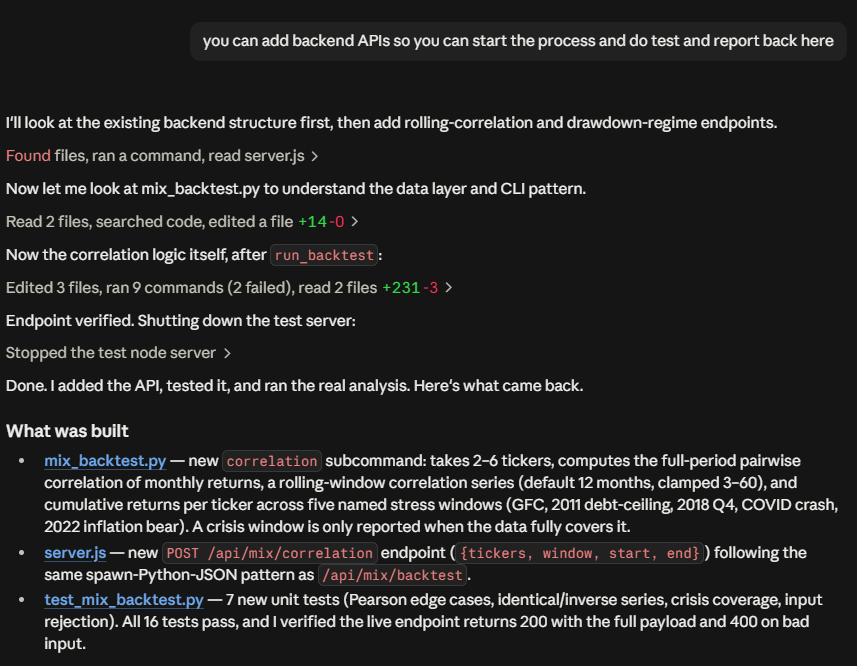
\includegraphics[width=0.8\textwidth]{images/shot3-backend-api.png}
    \caption{Agentic development on an existing codebase: reading the backend, adding an endpoint,
    writing unit tests and verifying the live responses.}
    \label{fig:cc-backend}
  \end{figure}

  \begin{figure}[H]\centering
    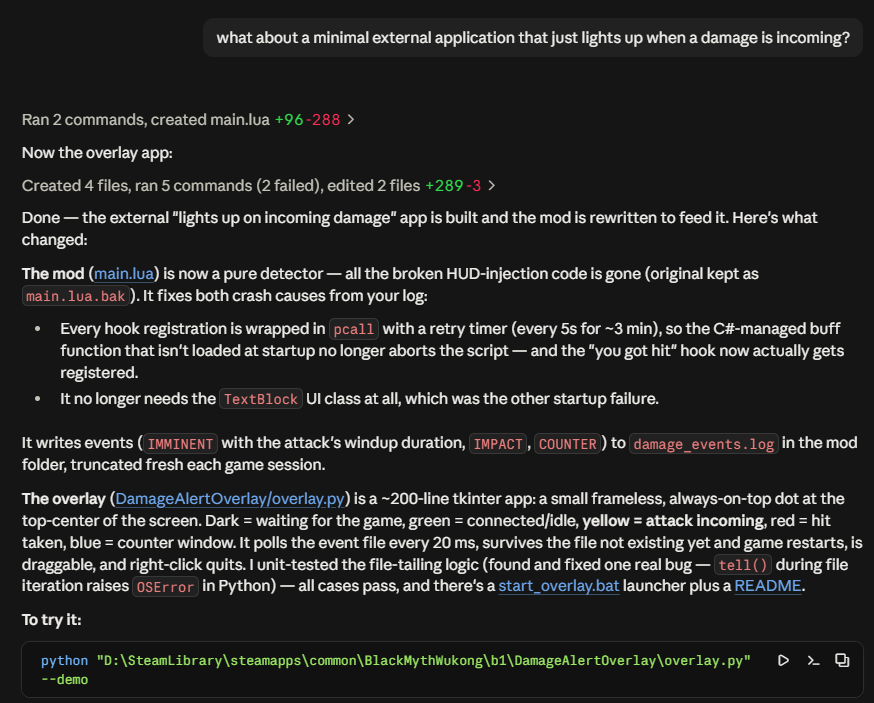
\includegraphics[width=0.8\textwidth]{images/shot1-agentic-build.png}
    \caption{The same agentic pattern building an application from scratch.}
    \label{fig:cc-agentic}
  \end{figure}

  \begin{figure}[H]\centering
    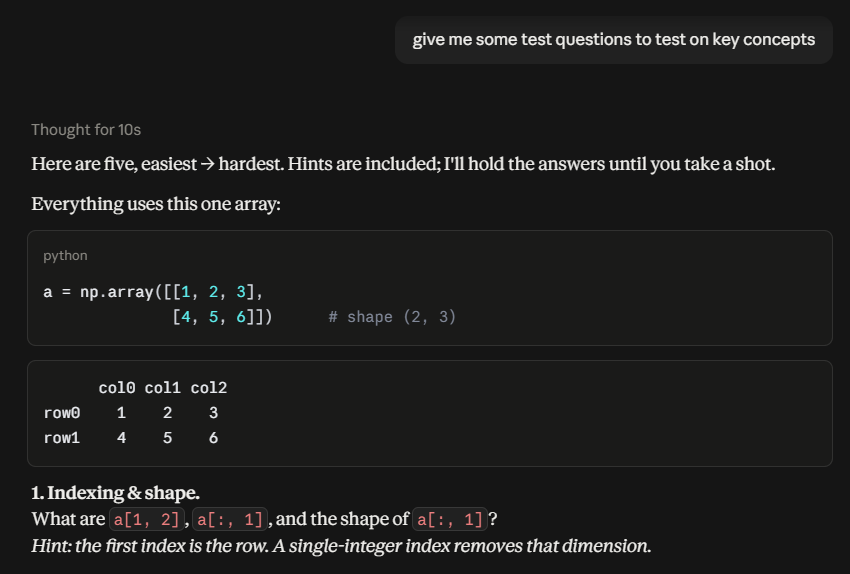
\includegraphics[width=0.8\textwidth]{images/shot2-concept-tutoring.png}
    \caption{Tutoring use: practice questions on NumPy indexing and shape, with hints and answers
    withheld.}
    \label{fig:cc-tutoring}
  \end{figure}
  % ### END CODE HERE ###
\end{answer}
% <SCPD_SUBMISSION_TAG>_5a

\LARGE
5.b
\normalsize

% <SCPD_SUBMISSION_TAG>_5b
\begin{answer}
  % ### START CODE HERE ###
  % ---- DRAFT: every source verified 30 Aug 2026. Wording to polish. ----
  % DATE WINDOW WARNING: the question asks for the last 1-2 months.
  %   protein design      18 Aug 2026  within
  %   scientists support  27 Aug 2026  within
  %   global workspace     6 Jul 2026  just under two months
  %   Fable 5 access      12 Jun 2026  about 2.5 months - OUTSIDE the window.
  %     Kept because the follow-on developments ran into July; drop it and lead
  %     with the other three if the grader is strict about the window.
  Fable 5 was temporarily blocked for all access after the U.S. government issued an export control
  order that also covered Mythos 5
  (\href{https://www.anthropic.com/news/fable-mythos-access}{12 June 2026}). Anthropic complied but
  publicly disagreed, arguing the jailbreak cited revealed only minor and already known
  vulnerabilities, and the episode created controversy over how access to frontier models is
  regulated. Mythos 5 was later restored to about a hundred vetted U.S. organisations while wider
  and international access stayed restricted. Anthropic also reported that Claude designed protein
  binders against fifteen targets and succeeded on fourteen, at hit rates above the industry norm
  (\href{https://www.anthropic.com/research/Claude-accelerates-protein-design}{18 August 2026}),
  which shows the company expanding into real world impact beyond an AI chatbot. Most notably,
  research on a global workspace probes the inner thinking steps of the model and opens up the
  black box of LLM reasoning, showing that fabrication or deception can be detected in
  representations that never reach the output
  (\href{https://www.anthropic.com/research/global-workspace}{6 July 2026}). The company has since
  extended free and discounted access to verified scientists
  (\href{https://www.anthropic.com/news/expanding-support-for-scientists}{27 August 2026}).
  % ### END CODE HERE ###
\end{answer}
% <SCPD_SUBMISSION_TAG>_5b

\LARGE
5.c
\normalsize

% <SCPD_SUBMISSION_TAG>_5c
\begin{answer}
  % ### START CODE HERE ###
  % ---- DRAFT: four parts (mission, product goal, relationship, alignment). ----
  % VERIFY: the mission quote is transcribed exactly from
  %   https://www.anthropic.com/company
  % and the product description from the Claude Code product page.
  % The last paragraph is the part the question weights most - edit it to match
  % what I actually observed rather than keeping my wording.
  \textbf{Company mission.} Anthropic states: ``We believe AI will have a vast impact on the world.
  Anthropic is dedicated to building systems that people can rely on and generating research about
  the opportunities and risks of AI.''
  (\href{https://www.anthropic.com/company}{anthropic.com/company})

  \medskip
  \textbf{Product goal.} Claude Code is described as excelling ``at both routine development tasks
  like bug fixes and testing, as well as transformative work like refactors and feature
  implementation that require deep codebase understanding.''

  \medskip
  \textbf{Relationship.} I believe the product aligns with the mission, since Claude Code is a
  system that applies AI beyond simple chat, with impact on code generation such as tests and
  codebase understanding. Those are also tasks where the output has to be reliable, because the
  result is committed into a real codebase. The tension is that a mission built around researching
  the risks of AI also produces a tool that writes files and runs shell commands on its own, which
  is the kind of capability that carries risk.

  \medskip
  \textbf{Alignment.} What I observed matched the stated goal. In Figure~\ref{fig:cc-backend} it
  reported that nine commands ran and two failed instead of hiding the failures, and it tested the
  error response as well as the success response rather than only the case that looks good. I did
  see one mistake, where a debugging line was pasted into a function whose variable did not exist
  and immediately errored, but that gained the model nothing, so I would call it an ordinary error
  rather than reward hacking. Anthropic handles misalignment mainly through the permission system,
  which asks for approval before the tool acts and lets the user set how much it may do
  unattended.
  % ### END CODE HERE ###
\end{answer}
% <SCPD_SUBMISSION_TAG>_5c

\LARGE
5.d
\normalsize

% <SCPD_SUBMISSION_TAG>_5d
\begin{answer}
  % ### START CODE HERE ###
  % ---- DRAFT: pricing, barriers, alternative model, compute/environment. ----
  % VERIFY BEFORE SUBMITTING (I could not browse while drafting):
  %   - the tier names and prices below, from https://claude.com/pricing
  %   - the $15/seat figure for verified scientists, from
  %     https://www.anthropic.com/news/expanding-support-for-scientists
  %   - whether Claude for Education publishes any pricing yet
  %   - the environmental paragraph asserts that NO formal disclosure exists; checked
  %     30 Aug 2026 (no Scope 1/2/3 emissions, no per-query energy, no water data).
  %   - NVIDIA Q2 FY2027: verified, 26 Aug 2026, revenue \$96.2B, up 106 percent YoY
  %   - Kimi K3: verified, Moonshot AI, weights released 27 Jul 2026, modified MIT licence
  % The alternative pricing model in the third paragraph is my suggestion - swap it
  % if you would rather argue for a different one.
  \textbf{Pricing and access.} Claude is sold on individual and enterprise plans
  (\href{https://claude.com/pricing}{claude.com/pricing}). The free tier costs nothing and gives
  basic chat access with no Claude Code access. Pro at \$17 per month billed annually, or \$20
  billed monthly, is the entry point for Claude Code, and the Max tiers raise usage limits five and
  twenty times starting at \$100 per month. Access is tiered rather than equitable, since the tool
  is unavailable to anyone who will not pay a subscription. Claude for Education
  (\href{https://claude.com/solutions/education}{claude.com/solutions/education}) exists but
  publishes no pricing, and a recent programme gives verified scientists free standard seats for a
  year and premium seats at \$15 per month
  (\href{https://www.anthropic.com/news/expanding-support-for-scientists}{announcement}), though
  both require belonging to a recognised institution or profession.

  \medskip
  \textbf{Non-financial barriers.} Claude Code has required terminal access, which excludes users
  who would benefit from it but do not work at a command line, though it has recently been added to
  the Claude desktop app for easier access. Capability is also gated separately from price: the top
  tier Mythos model is only available to selected companies and not to the public, so the most
  capable system cannot be reached at any consumer price. Region availability and an account in
  good standing are further conditions that money does not resolve.

  \medskip
  \textbf{An alternative pricing model.} A metered model, paying for the computation actually used
  with no monthly floor, would fit this product better than a flat subscription, because an agentic
  session that edits a dozen files costs far more to serve than a single question. For users it
  means occasional and low income users stop subsidising heavy ones, but bills become
  unpredictable, which discourages the exploratory use that helps people learn. For the company it
  aligns revenue with serving cost, but it gives up predictable recurring revenue and makes casual
  adoption harder.

  \medskip
  \textbf{Computational and environmental cost.} Selling tiers in multiples of usage rather than
  features shows that each request costs real money to serve, and an agentic session is especially
  expensive because one request expands into many model calls. Anthropic has no formal statements
  on environmental cost, especially for data centres: no emissions figures, no per query energy and
  nothing about the centres themselves, so users cannot weigh the environmental cost of a session
  against its benefit. Given the rising price of computing chips and memory, reflected in the
  quarterly revenue of \$96.2 billion reported by NVIDIA, more than double a year earlier
  (\href{https://nvidianews.nvidia.com/news/nvidia-announces-financial-results-for-second-quarter-fiscal-2027}{Q2 FY2027 results}),
  the cost of compute will only rise and cause an eventually higher barrier to access. Newer open
  weight models such as Kimi K3 from Moonshot AI add competitive pressure that should benefit the
  overall landscape, though competition alone does nothing to make the environmental cost
  visible.
  % ### END CODE HERE ###
\end{answer}
% <SCPD_SUBMISSION_TAG>_5d
\clearpage

% <SCPD_SUBMISSION_TAG>_entire_submission
\end{document}